\documentclass[a4paper,12pt]{article}

\usepackage[utf8]{inputenc}
\usepackage{graphicx}
\usepackage{titletoc}
\usepackage{lipsum}
\usepackage{listings}
\usepackage{filecontents}
\usepackage{subcaption}

\usepackage[top=2.5cm, bottom=2.5cm, left=2.5cm, right=2.5cm]{geometry}

\lstset{
  basicstyle={\ttfamily},
  identifierstyle={\small},
  commentstyle={\smallitshape},
  keywordstyle={\small\bfseries},
  ndkeywordstyle={\small},
  stringstyle={\small\ttfamily},
  frame={tb},
  breaklines=true,
  columns=[l]{fullflexible},
  numbers=left,
  xrightmargin=0zw,
  xleftmargin=3zw,
  numberstyle={\scriptsize},
  stepnumber=1,
  numbersep=1zw,
  lineskip=-0.5ex
}

\title{DPマッチングによる単語音声の認識}
\author{麻生英寿 \\ 21C1005}
\date{\today}

\begin{document}

\maketitle

\tableofcontents

\section{目的}

DPマッチングのアルゴリズムを利用して,小語彙の音声認識の実験を行う.

\section{実験方法}

DPマッチングのアルゴリズムによって音声データの単語間距離を計算するプログラムを作成する.
そのプログラムに,100単語の音声データのテンプレートに対して,同じ発声内容の100単語を未知入力音声として,順に入力していく.
入力された音声データの発声内容を判定し,その正答率を計算する.

\subsection{使用したデータセットについて}

この実験で使用した音声データセットには,2人の話者がそれぞれ同じ100種類の単語を発話したものが含まれている.
話者は100種類の単語の発話を2回行っているため,合計400個の音声データが含まれている.
1つの音声データにはファイル名,発声内容,フレーム数とフレーム数分の15次のメルケプストラム特徴量である.

\subsection{単語間距離の計算}

実験ではDPマッチングのアルゴリズムを用いて2つの音声データの単語間距離を計算する.
単語間距離の計算は以下の手順で行う.

入力として与えられた2つの音声データのフレーム長をそれぞれ$I$と$J$とする.
$(i,j),0<i\leq I ,0<j\leq J$で表せられる2つの音声データの各ノードのメルケプストラム特徴量の距離を計算し,
$(i,j)$でのフレームの距離を局所距離$d(i,j)$と表す.
音声データの最初のフレームから任意のフレームまでの局所距離の総和を累積距離$g(i,j)$とする.
最終フレームでの累積距離$g(I,J)$が最小となるような経路を探索することで,単語間距離を計算する.

\subsection{最終フレームでの累積距離の計算}

はじめに,初期条件を以下のように設定する.
\[
    g(0,0) = d(0,0)
\]
次に境界条件を以下のように設定する.
\[
    j>0 \rightarrow g(0,j) = g(0,j-1) + d(0,j)
\]
\[
    i>0 \rightarrow g(i,0) = g(i-1,0) + d(i,0)
\]
最後に,再帰的に以下の式を用いて,最終フレームでの累積距離$g(I,J)$を計算する.
\[
g(i, j)=\min \left[\begin{array}{llr}
g(i, j-1) & + & d(i, j) \\
g(i-1, j-1) & + & 2 d(i, j) \\
g(i-1, j) & + & d(i, j)
\end{array}\right]
\]

\section{実験結果}
音声認識の正答率は\ref{tab:correct}の通りである.

\begin{table}[htbp]
    \centering
    \begin{tabular}{|c|c|c|c|c|}
      \hline
      モデル/認識対象 & city011 & city012 & city021 & city022 \\
      \hline
      city011 &       & 99\% & 90\%  & 84\% \\
      \hline
      city012 & 100\% &      & 92\%  & 86\% \\
      \hline
      city021 & 83\%  & 91\% &       & 99\% \\
      \hline
      city022 & 86\% &  94\% & 100\%  &      \\
      \hline
    \end{tabular}
    \caption{音声認識の正答率}
    \label{tab:correct}
\end{table}


\newpage

\section{考察}
実験結果より,同一話者よりも異なる話者の音声データの方が正答率が低いことが読み取れる.
これは,同一話者の音声データの方が,異なる話者の音声データよりも似ているため,
プログラムによって求められた単語間距離も小さくなり,正答率が高くなったと考えられる.

ここで話者や発声単語の違いが正答率に与える影響を調べるために,累積距離を可視化してみる.
同じ音声データ,同じ話者,異なる話者,異なる話者かつ異なる発声単語の4通りの音声データの組み合わせでの
累積距離を図\ref{fig:equal},図\ref{fig:same},図\ref{fig:diffpeople},図\ref{fig:diffword}に示す.

\begin{figure}[h]
    \centering
    \begin{subfigure}[b]{0.45\textwidth}
      \centering
      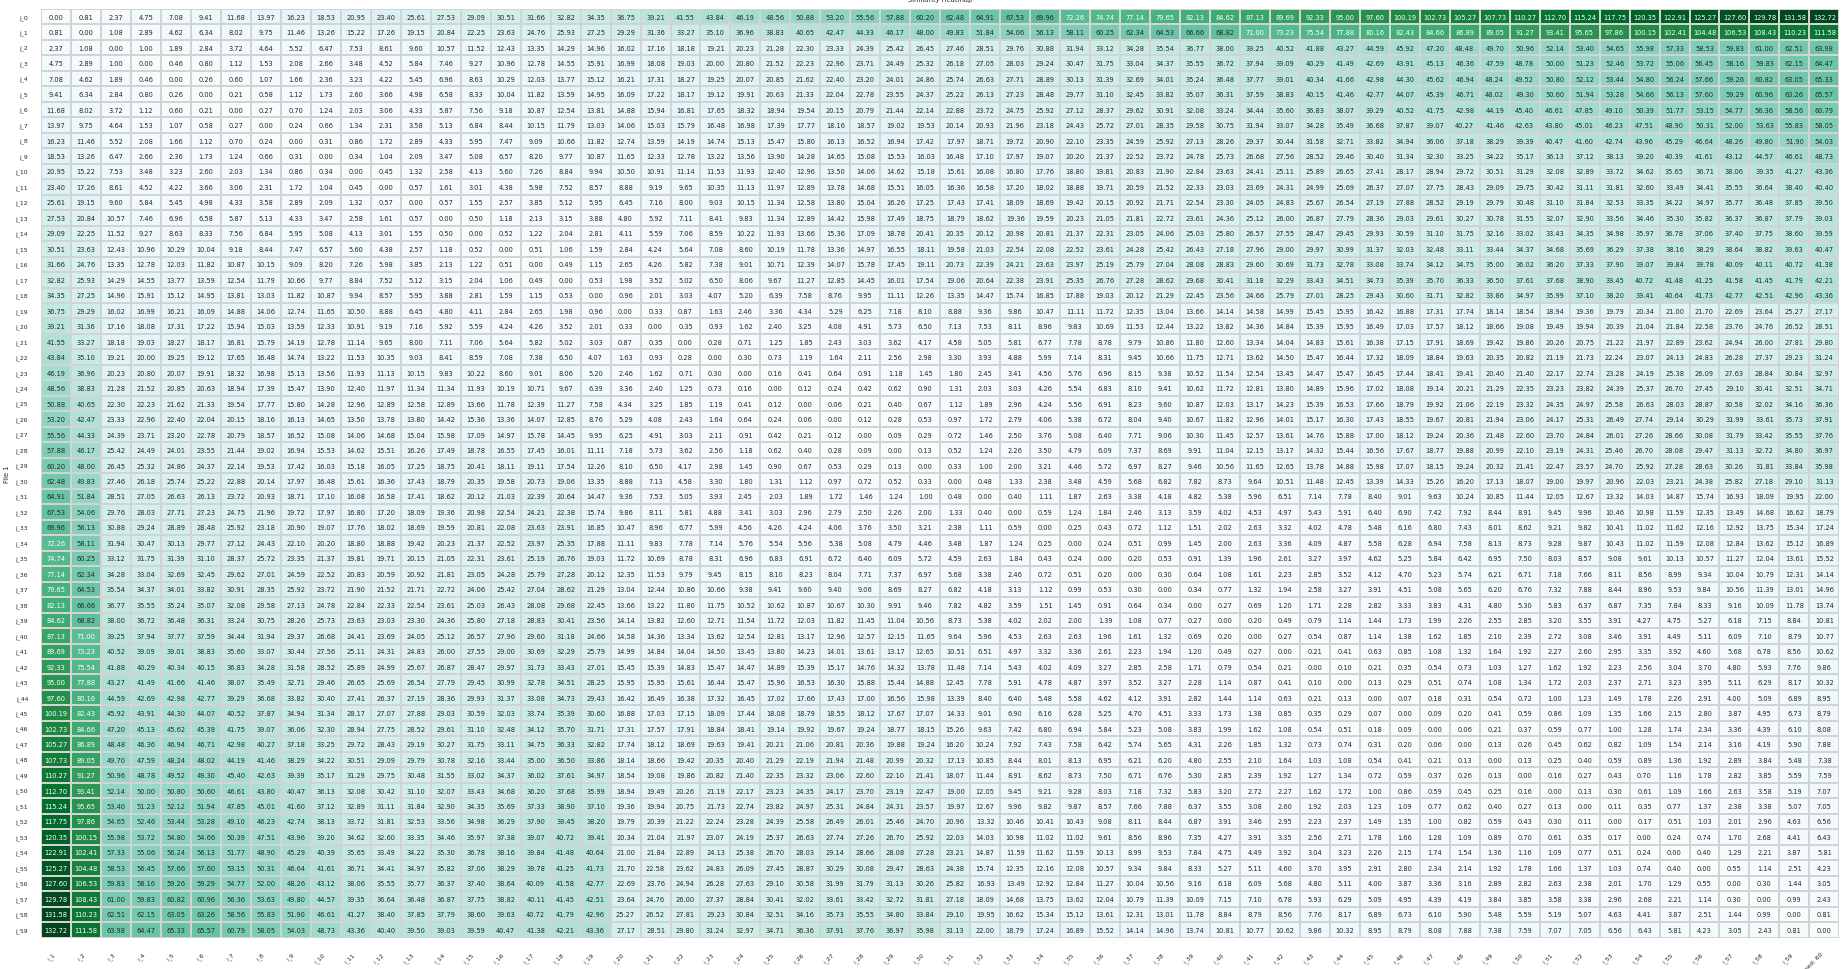
\includegraphics[width=\textwidth,bb=0.000000 0.000000 1329.122658 697.681395]{./equal.png}
      \caption{city011\_001 \& city011\_001}
      \label{fig:equal}
    \end{subfigure}
    \hfill
    \begin{subfigure}[b]{0.45\textwidth}
      \centering
      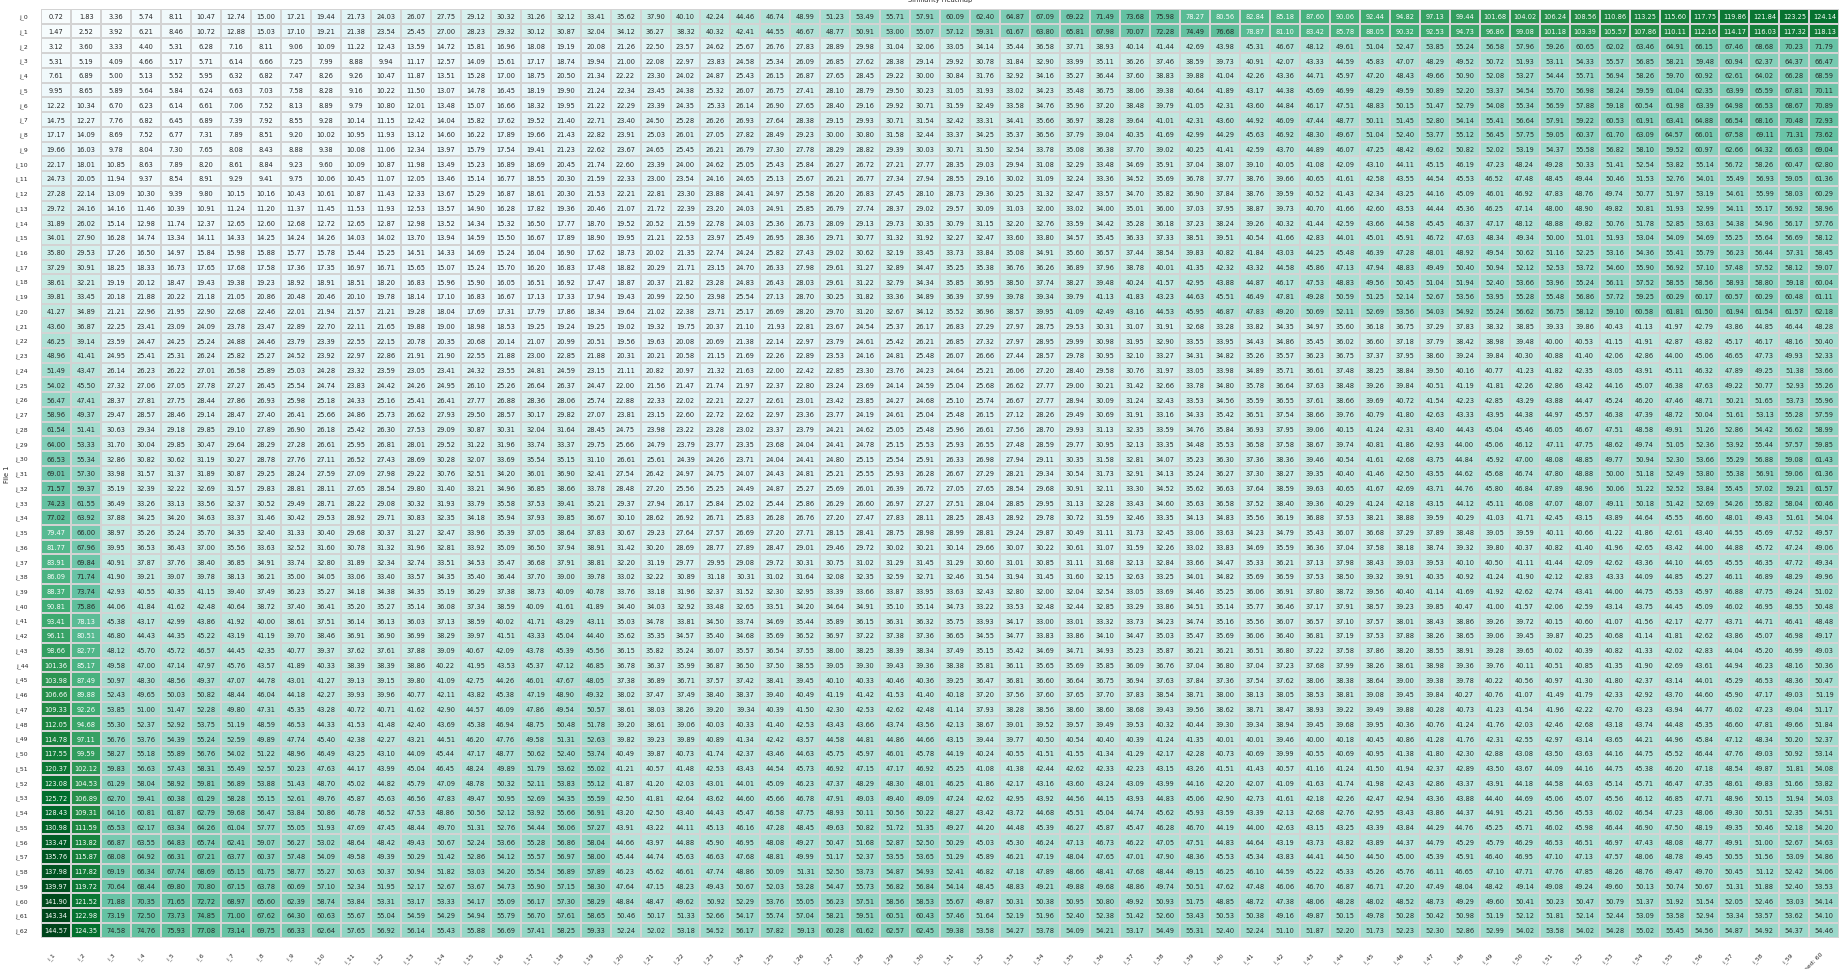
\includegraphics[width=\textwidth,bb=0.000000 0.000000 1329.122658 697.681395]{./same.png}
      \caption{city011\_001 \& city012\_001}
      \label{fig:same}
    \end{subfigure}
  
    \vspace{0.5cm} % 行間のスペース調整
  
    \begin{subfigure}[b]{0.45\textwidth}
      \centering
      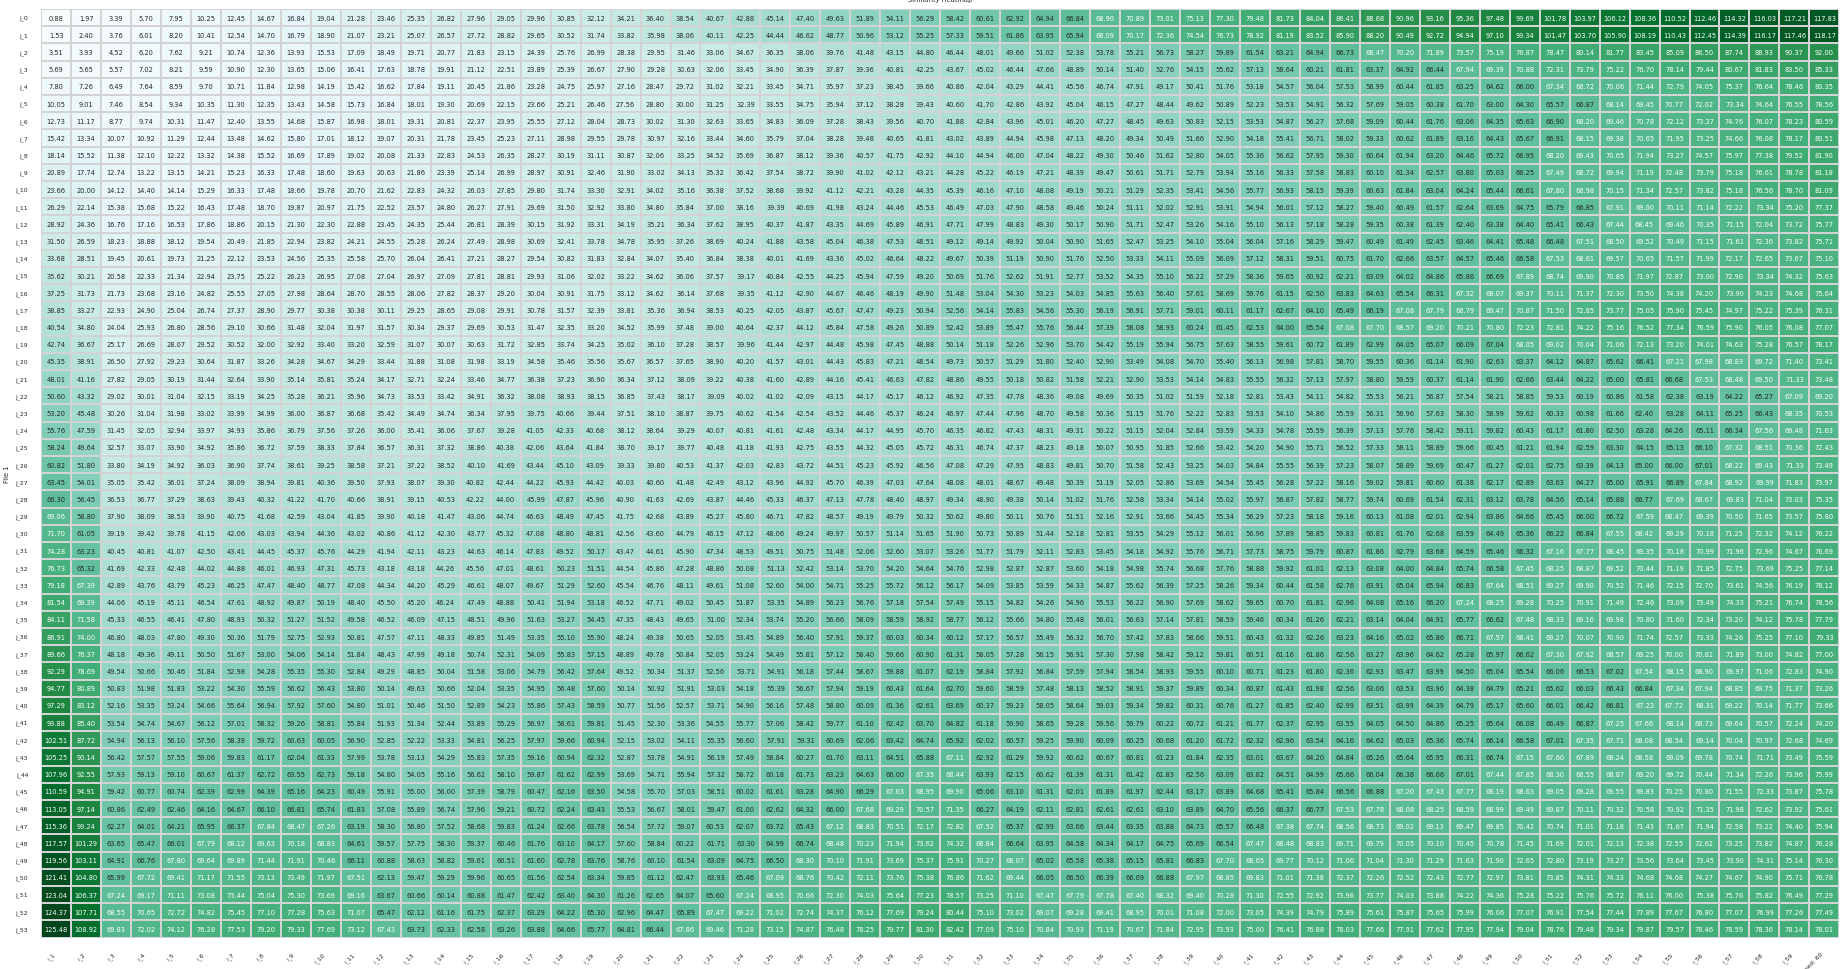
\includegraphics[width=\textwidth,bb=0.000000 0.000000 1329.122658 697.681395]{./diffpeople.png}
      \caption{}
      \caption{city011\_001 \& city021\_001}
      \label{fig:diffpeople}
    \end{subfigure}
    \hfill
    \begin{subfigure}[b]{0.45\textwidth}
      \centering
      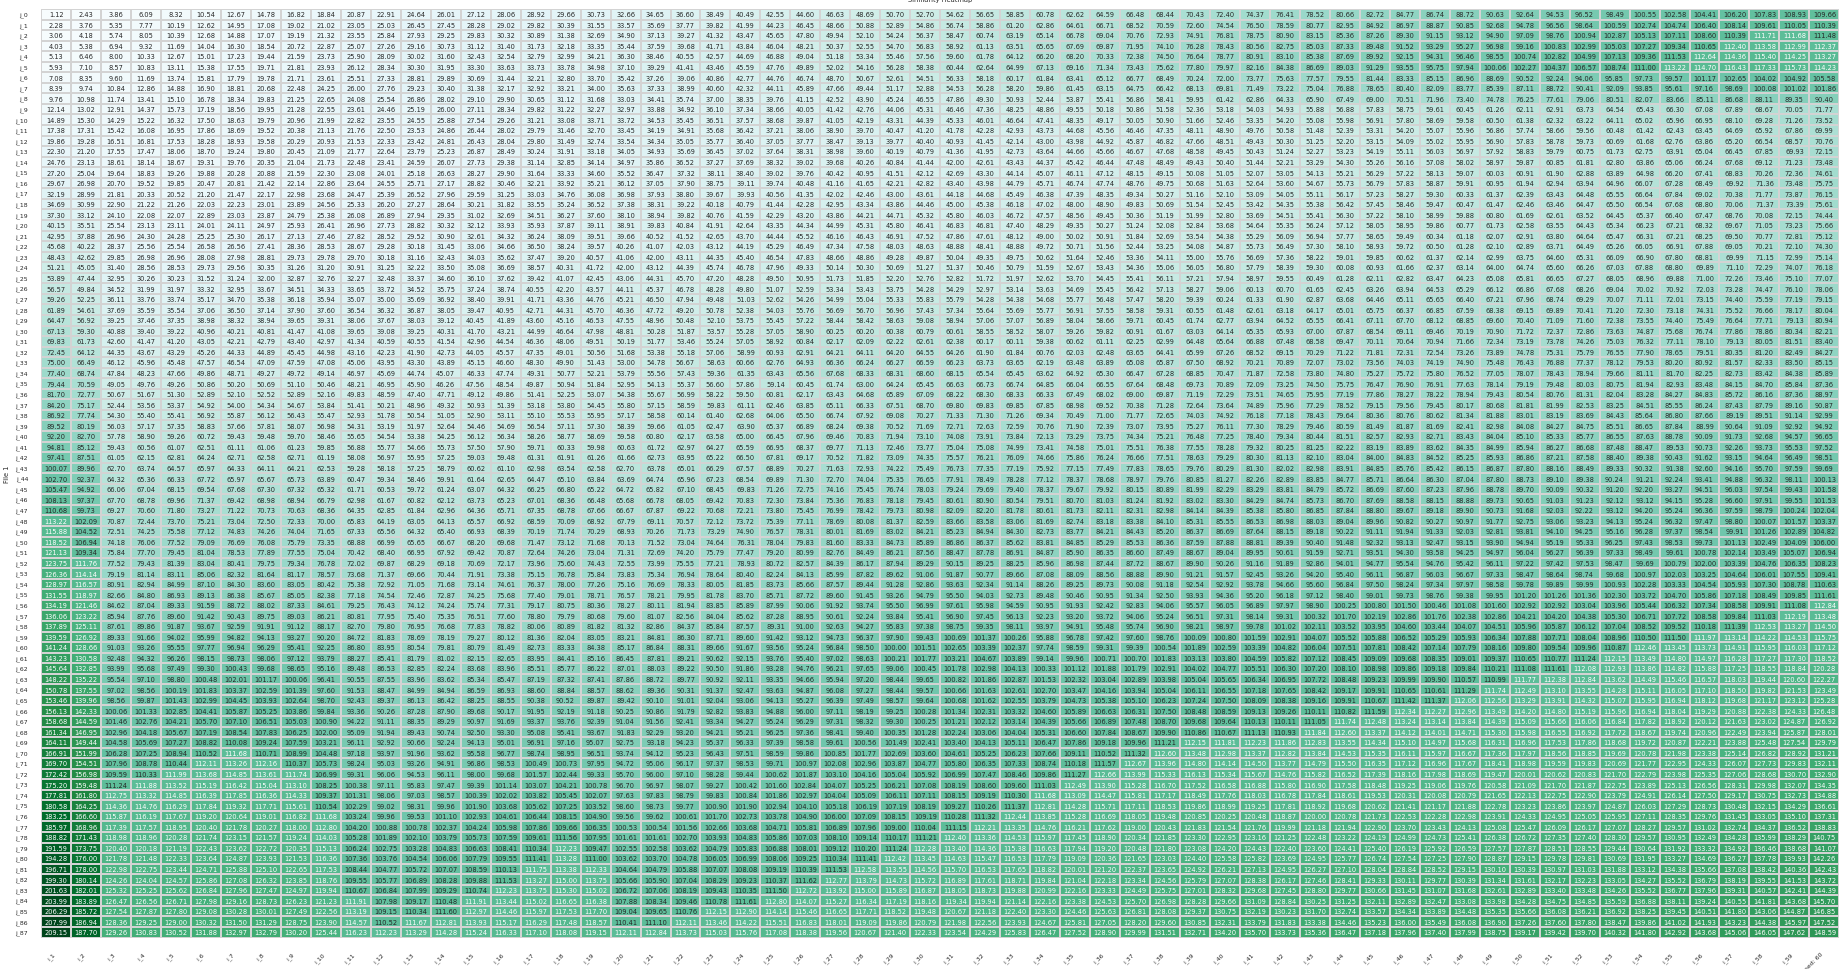
\includegraphics[width=\textwidth,bb=0.000000 0.000000 1329.122658 697.681395]{./diffword.png}
      \caption{city011\_001 \& city021\_011}
      \label{fig:diffword}
    \end{subfigure}
  
    \caption{累積距離のマップ}
    \label{fig:grid}
\end{figure}

これらの図は縦軸と横軸がそれぞれ入力音声データのフレームを表していて,各々のマスの濃淡はそのノードでの累積距離を表している.
色が濃いほど累積距離が大きく,色が薄いほど累積距離が小さいことを意味する.
同じ発声内容である,図\ref{fig:equal}と図\ref{fig:same},図\ref{fig:diffpeople}では,図の左上と右下の対角線で色の分布が線対称になっている.
しかし,同じ音声データ,同じ話者,異なる話者とデータの違いが大きくなるごとに,対称性が失われていることがわかる.
発声内容が異なる図\ref{fig:diffword}に至っては,対称性が明らかに失われている.

\newpage

\appendix
\section{付録}
この実験で使用したプログラムのソースコードを以下に示す.

\subsection{付録A: 単語間距離を求めるプログラム}
\lstinputlisting[language=c]{../two_words.c}

\subsection{付録B:正答率を計算するプログラム}
\lstinputlisting[language=c]{../benchmark.py}

\subsection{付録C:可視化するプログラム}
\lstinputlisting[language=c]{../heatmap.py}



\end{document}
